%% Only upto line 66, modifications have been done
%\documentclass[12pt, Arial]{article}    %%%%Helvetica
%%%\documentclass[12pt]{article}
%\usepackage{epsfig}
%\usepackage{cite}
%\usepackage{times}
%\usepackage{amsmath}
%\usepackage{amssymb}
%\usepackage{subfigure}
%\setlength{\textheight}{9.6in}
%\setlength{\textwidth}{6.8in} \setlength{\oddsidemargin}{-0.04in}
%\setlength{\headheight}{0.0in} \setlength{\headsep}{0.15in}
%\setlength{\topmargin}{0.5cm}
%%\setlength{\parskip}{0.25in}
%\renewcommand{\baselinestretch}{1.2}
%\begin{document}
\thispagestyle{empty}
% cover page
\vspace{.5in} \centerline{\huge{\textbf{Synopsis}}}
%%\begin{center}
%%\LARGE{Multiscale Processing of Multichannel Electrocardiogram
%%Signals}
%%\end{center}
\vspace{0.5in}
%\centerline{\LARGE{ \emph{}}}
%\vspace{0.15in} \centerline{\large{\em A THESIS to be submitted by}}
%\vspace{0.3in} {\centerline {\large{\LARGE L. N. Sharma}}} \vspace{0.2in} \vspace{0.1in} \centerline{\large{\em
%for the award of the degree}} \vspace{0.1in} \centerline{
%\emph{of} } \vspace{0.2in} \centerline{\LARGE DOCTOR OF
%PHILOSOPHY} \vspace{0.3in}\centerline{\large{\em supervisors}}
%\vspace{0.2in} \centerline{\large{Prof. S. Dandapat and Prof. A. Mahanta }}
%\vspace*{1in}
%\begin{figure}[!hbt]
%\centerline{\epsfig{figure=IITGC.eps,scale=0.20}}
%\end{figure}
%\vspace{0.1in} \centerline {\large{\textsf{DEPARTMENT OF
%ELECTRONICS AND ELECTRICAL ENGINEERING}}}
%\vspace{0.05in}\centerline {\large{\textsf{INDIAN INSTITUTE OF
%TECHNOLOGY GUWAHATI}}} \vspace{0.05in}\centerline
%{\large{\textsf{GUWAHATI-781 039, INDIA.}}}
%\vspace{0.1in}\centerline{\textsf{ December 2011.}}
%\thispagestyle{empty}
%\newpage
%\setcounter{page}{1}
%\section{Introduction}


\noindent \textbf{\Large{Introduction}}
\vspace{0.2in}

\noindent This thesis work is an investigation of multichannel
electrocardiogram (ECG) signal processing using wavelets. Cardiac
signal processing aims at extracting significant information from
ECG signals for diagnosis, therapy and monitoring. Multi-lead or
Multichannel Electrocardiogram (MECG) signals  are essential for a
physician to make a critical diagnostic decision for a cardiac
patient. In case of clinical evaluation, $12$-lead standard ECG
recording view the heart at different angles. This gives
spatio-temporal distribution of electrical potential of heart. Due
to its special nature, such signals need to be addressed with care
during their processing. Processing of these signals should
preserve the clinically important information and relevant
diagnostics features. A good amount of temporal correlation exists
in a single channel ECG. Also, the inter-lead correlation is high
in a multichannel channel ECG signal. These correlation properties
can be exploited for efficient implementation of algorithms for
multichannel ECG signal processing.

This work consists of three major contributions. First, for
preprocessing of ECG signals, wavelet based denoising methods are
proposed and evaluated for noise cancellation. The proposed
denoising methods are based on relative subband energy of the
signal and its Gaussianity from real data. Higher order statistics
at different wavelet subbands provides significant information
about the statistical nature of the data in time and frequency.
The fourth order cumulant, Kurtosis, and the Energy Contribution
Efficiency (ECE) of signal in a wavelet subband are combined to
assess the noise content in the signal. Second, Multiscale
Principal Components Analysis (MSPCA) is investigated for
compression of multichannel electrocardiogram signals.  The higher
correlations between multichannel ECG signal-components at similar
wavelet scales help reduce dimension and remove redundant
information present in signals. Using covariance method  for PCA,
it is found that the proposed method perform data dimension
reduction without introducing distortion on clinical information.
Multichannel compression is implemented using uniform quantizer
and entropy coding of MSPCA coefficients. Third, Clinical Entropy
(Centropy) is proposed   based on an information theoretic
approach to eigenvalue matrices resulted from MSPCA. It is shown
that Centropy can effectively quantify the  distortions in the
clinical components in an ECG signal.

%%\section{Motivation}

\vspace{0.3in}
\noindent \textbf{\Large{Motivation}}
\vspace{0.2in}

\noindent The cardiac potentials recorded using multiple leads on
human body represent the same cardiac event at different spatial
locations. The same electrical pulse originating from sinus node
creates `PQRST' morphologies and appears in different ECG
channels. Thus, the signals at different leads are highly
correlated. The individual components, P-wave, QRS-complex and
T-wave, of an ECG do have different frequency contents.
Multiresolution decomposition segments these components or
information broadly in different frequency bands. It is expected
that, at a wavelet scale, inter-lead correlation may be high.

\begin{figure}[!ht] \center
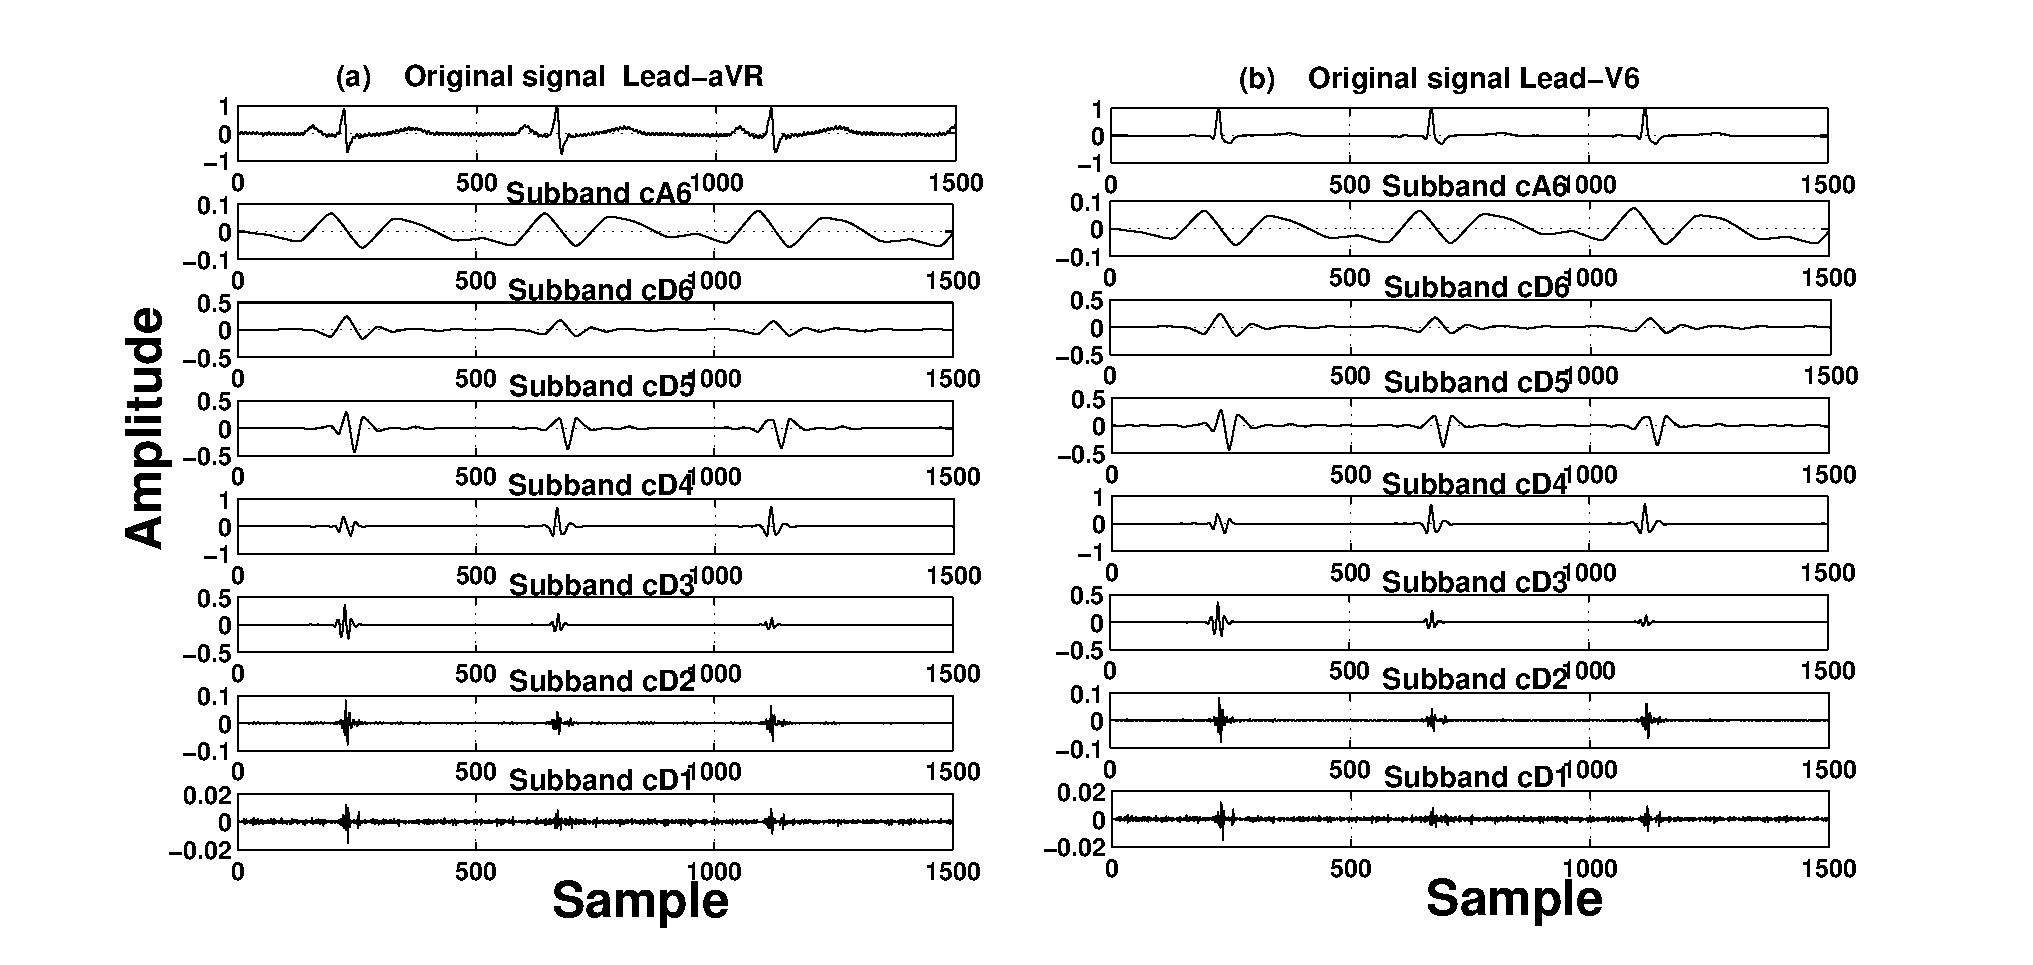
\includegraphics[height=4.1in,width=6.9in]{TimeM041-aVR-V6.eps}
\caption*{\textbf{Figure:} Original time domain Lead-aVR and V6
signals and their reconstructed subbands signals due to six level
wavelet decomposition. In panels, (a) Original Lead-aVR signal
with reconstructed subband signals and (b) Original Lead-V6 signal
with reconstructed subband signals. Data base used is from CSE
multilead measurement library, Data set:
MO1-041}\label{Corr-subbands-aVR-V6}
\end{figure}

In Figure above, wavelet subband signals with original signals are
shown for Lead-aVR and Lead-V6. It is observed that cA6 subband
reflects the parts of low frequency components such as P-wave and
T-wave in leads (Figure (a) and (b)). The cD6 and the cD5 subbands
show the lower frequency component of QRS-complex with higher
frequency component of T-wave. The cD4 and the cD3 subbands show
the significant higher frequency component of QRS-complex. The cD2
and the cD1 subbands contain some higher frequency component of
QRS-complex and noise. It is seen that in same subband levels or
scales, in both the cases, there are similarities between
segmented signal components. So, it is expected to get higher
correlation between different channels in the same subband level.
If all the channels of a standard 12-lead ECG are subjected to
wavelet transform with the same decomposition level and mother
wavelet, it is expected that, at a wavelet scale, inter-lead
correlation may be much higher.

So, there is a scope of applying multivariate data analysis method
at a wavelet scale if the coefficients of all the channels are
organized as multivariate data. These multivariate data are
expected to show higher inter-channel redundancies at a wavelet
scale. Also, it is expected to have similar pattern of multiscale
energy for multivariate data. Based on these assumptions,
dimensions can be reduced applying principal component analysis
(PCA) at wavelet scales for non-significant multivariate data.

%%\section{Preprocessing of Multichannel Electrocardiogram Signal} \label{preprocess-MECG}
\vspace{0.3in} \noindent \textbf{\Large{Preprocessing of
Multichannel Electrocardiogram Signals}} \label{preprocess-MECG}
\vspace{0.2in}

\noindent Preprocessing of an ECG signal consists of  noise
cancellation and amplitude and time normalization. In this work,
noise cancellation of multichannel ECG data using wavelets is
dealt as a preprocessing problem. Processing of ECG signals should
preserve the clinically important information and relevant
diagnostics features. Though the ECG signal denoising is an old
problem, still there should be special consideration to ensure
signal fidelity for retention of clinical information. In this
work, two novel denoising methods are proposed. The first method
is based on evaluation of higher order statistics at different
wavelet subbands for an electrocardiogram (ECG) signal. Higher
order statistics at different wavelet subbands provides
significant information about the statistical nature of the data
in time and frequency. The fourth order cumulant, Kurtosis, and
the Energy Contribution Efficiency (ECE)  of signal in a wavelet
subband are combined to assess the noise content in the signal.
Accordingly, four denoising factors are defined. Performance of
the denoising factors are evaluated and compared with the soft
thresholding method. The filtered signal quality is assessed using
Percentage Root Mean Square Difference (PRD), Wavelet Weighted
Percentage Root Mean Square Difference (WWPRD), Wavelet
Energy-based Diagnostic Distortion (WEDD) measures. It is observed
that the proposed denoising scheme not only filters the signal
effectively but also help retain the diagnostic information.

The second denoising method is based on a threshold which is derived
by considering energy contribution of a wavelet subband, noise
variance which is based on a  Gaussian measure, Kurtosis, and
number of samples. The robust noise estimator, median absolute
deviation (MAD), is scaled by a normalized wavelet subband
Kurtosis instead of conventional statistical quantile function for
Gaussian distribution.
The method is
tested with spatially nonhomogeneous functions, Blocks, Bumps,
HeaviSine and Doppler with noise. The performance of the proposed
thresholding method is evaluated using synthetic ECG signal after
adding noise and the recorded noisy ECG signal from database. Also, it is
compared with the existing classical thresholding methods such as
soft thresholding, hard threshoding and SURE. The lowest
PRD, WWPRD and WEDD values are achieved as $9.523\%$, $17.743\%$
and $4.000\%$ for lead-V2, lead-V3 and lead-II signal respectively.  Results show that
the performance of the proposed method is better compared to the
existing methods. The proposed denoising method not only filters
ECG signal effectively but also can help retain the clinical
information in the signal.

\vspace{0.3in}
%%%\section{Multiscale PCA for Multichannel ECG Compression}
\noindent \textbf{\Large{Multiscale PCA for Multichannel ECG
Compression}} \label{MSPCA-MECG}
\vspace{0.2in}

\noindent Cardiac signal-components (P-wave, QRS-complex and
T-wave) are grossly segmented to different wavelet subbands. In
wavelet subbands, the correlation between multichannel ECG
signal-components can be effectively captured. In this work, the
correlations across the ECG channels at the same wavelet scales
are investigated using scatter plots and correlation coefficients.
Higher correlation of multichannel ECG data in wavelet subbands
will help efficient implementation of PCA.   If there are $n$
number of ECG channels which are `$L$' level wavelet decomposed
and $j^{th}$ subband of all channels are collected in a matrix, it
forms `$L+1$' wavelet subband matrix. Multiscale wavelet subband
matrix for approximation band is $\mathbf{A_{L}}$ and subband
matrices for details are $\mathbf{D_{j}}$, where $j=1, 2, \cdots,
L$. In this, the number of columns is the number of ECG channels
and number of rows is the number of coefficients in that
particular subband.  The selection of principal components based
on subband energy is proposed.  It is based on average fractional
energy contribution of eigenvalue in a data matrix. It is seen
that the selected PC represent the clinical information while
discarding redundant information associated with non-significant
PC. For evaluation of clinical fidelity, quantitative measures
such as percentage PRD, WWPRD and WEDD are evaluated. The
dimension reduced signals fall under excellent category with
lowest WEDD value of $1.67\%$. The dimension reduction at
multiscale multivariate matrices gives an overall samples
reduction of $50.37\%$ for 12 channel ECG with an average PRD of
$10.01\%$. These results motivated us for developing a compression
scheme for multichannel electrocardiogram (MECG) data, using
multiscale principal component analysis (MSPCA).  Multichannel
compression is implemented using uniform quantizer and entropy
coding of PCA coefficients.  Using data set from CSE mutlilead
measurement library, multichannel compression ratio of 5.98:1 is
found with PRD value 2.09\% and the lowest WEDD value of 4.19\%.
Based on, gold standard subjective quality measure, the lowest
mean opinion score (MOS) error value of $5.56\%$ is found.


%%\section{Clinical Entropy based MSPCA and Multiscale Distortion}
\vspace{0.3in}
\noindent \textbf{\Large{Clinical Entropy based MSPCA and Multiscale
Distortion}}
\vspace{0.2in}

\noindent A novel MSPCA based clinical entropy measure is proposed
to evaluate the clinical information in the processed signal.
Higher correlation between different channels in the same subband
level help efficient implementation of PCA at the subband level.
The eigenvalues at different wavelet scales capture the energy of
the multichannel signal. Also, the gross segmentation of different
ECG components in wavelet scales help capture of clinical
information through these eigen values. Clinical entropy is
investigated from the diagonal eigenvalue matrix. Centropy based
PC selection may be applied in PCA and MSPCA based processing of
multichannel ECG signals. Centropy based PCA is compared with
conventional PCA qualitatively and quantitatively evaluated using
distortion metrics, PRD, Root Mean Square Error (RMSE) and Cross
Correlation (CC) for all 12 channel data. It is observed that the
PRD and the RMSE values are lower for all the channels in case of
the proposed Centropy based PCA method compared to the
conventional PCA based method. Also, the compressed signals after
Centropy based PCA and Centropy based MSPCA are compared. For
Centropy based MSPCA method, the PRD, WWPRD and WEDD values for
lead-III signal are $11.725\%$ $29.124\%$ and $5.274\%$
respectively. The Centropy based method shows the best performance
over others. After reconstruction of MSPCA processed multichannel
signals, Multiscale Multivariate Distortion (MMD) is evaluated.
For Centropy based MSPCA (using same data set), if the threshold
is decided at 80\% of information, the MMD values for $D_{1}$,
$D_{2}$, $D_{3}$ $D_{4}$, $D_{5}$, $D_{6}$ and $A_{6}$ are
$79.92\%$, $45.48\%$, $63.89\%$, $2.14\%$, $2.08\%$, $1.93\%$, and
$2.07\%$ respectively. The average Multiscale Distortion (MD)
value is found as $0.5268\%$.

%%\section{Organization of the Thesis}
\vspace{0.3in}
\noindent \textbf{\Large{Organization of the Thesis}}
\vspace{0.2in}

\noindent The contents of the thesis are organized as: In
\textbf{Chapter 1}, introduction to ECG signals and its processing
in time, frequency and time-frequency domain are discussed with
published literatures. In \textbf{Chapter 2}, a related reviews of
wavelet transform based ECG signal processing is given. PCA based
processing and the motivation for this thesis work is discussed.
In \textbf{Chapter 3}, for preprocessing of multichannel ECG, two
novel ECG denoising methods are presented and evaluated. In
\textbf{Chapter 4}, multiscale PCA is introduced for multichannel
ECG signal processing. A compression scheme for multichannel ECG
using multiscale PCA is proposed. In \textbf{Chapter 5}, clinical
entropy based multiscale PCA and multiscale distortion measure are
introduced. Conclusion of the thesis is drawn in \textbf{Chapter
6} with major contributions from this thesis and scope for further
research.


\clearpage


%\noindent{\bf \LARGE Major References}
%\begin{enumerate}
%
%
%
%%----------------------------------------------------
%\bibitem{donoho95}
%D. L. Donoho,``De-noising by soft thresholding,'' \emph{IEEE
%Trans. Inform. Theory}, vol. 41, pp. 613 - 627, May 1995.
%
%\bibitem{donohojohn95}
%D. L. Donoho and I. M. Johnstone, ``Adapting to unknown smoothness
%via wavelet shrinkage,'' \emph{J. Amer. Statist. Assoc.}, vol. 90,
%pp. 1200 -1224, Dec. 1995.
%
%\bibitem{hong2007}
%Hoonbin Hong, Ming Liang, "K-Hybrid: A Kurtosis-Based Hybrid
%Thresholding Method for Mechanical Signal Denoising,"
%\emph{Transactions of the ASME}, vol. 129, pp. 458 - 470, August
%2007.
%
%
%\bibitem{Fahoum2006}
%Amjed S. Al-Fahoum,``Quality Assessment of ECG Compression
%Techniques Using a Wavelet-Based Diagonstic Measure",\emph{IEEE
%Trans. on Information Technology in Biomedicine}, vol.10, no.1,
%pp.182-191, Jan.2006.
%
%
%\bibitem{bakshi1998}
%B. R. Bakshi, ``Multiscale PCA with application to MSPC
%monitoring," \emph{AIChE Journal}, vol. 44, no. 7, pp.1596 - 1610,
%July 1998.
%
%\bibitem{bakshi1999}
%B. R. Bakshi,  ``Multiscale analysis and modeling using wavelets,"
%\emph{Journal of Chemometrics}, vol.13, pp.415 - 434, 1999.
%
%
%
%
%\item J. Chen, and S. Itoh, ``A wavelet transform-based ECG
%compression method guaranteeing desired signal quality,"
%\emph{IEEE Trans. Biomed. Eng.}, vol. 45, no. 12, pp. 1414-1419,
%Dec. 1998.
%
%
%\item   S. G. Miaou and H. L. Yen, ``A quality-on-demand algorithm
%for wavelet-based compression of electrocardiogram signals,"
%\emph{IEEE Trans. Biomed. Eng.}, vol. 49, no. 3, pp. 233-239,
%March 2002.
%
%
%\item A. Alesanco, S. Olmos, R. S. H. Istepanian, and J. Garcya,
%``Enhanced real-time ECG coder for packetized telecardiology
%applications," \emph{IEEE Trans. Inf. Technol. Biomed.}, vol. 10,
%no. 2, pp. 229-236, April 2006.
%
%
%\bibitem{mani2006}
%M.S.Manikandan and S. Dandapat, ``Wavelet threshold based ECG
%compression using USZZQ and Huffman coding of DSM,'' \emph{
%Journal of Biomedical Signal Processing and Control, Elsevier},
%vol.1, no.4, pp.261 - 270, 2006.
%
%\bibitem{mani2007}
%M.S.Manikandan and S. Dandapat, ``Wavelet energy based diagnostic
%distortion measure for ECG," \emph{ Journal of Biomedical Signal
%Processing and Control, Elsevier}, vol.2, pp.80 - 96, 2007.
%
%\bibitem{manisp2008}
%M.S.Manikandan and S. Dandapat, ``Multiscale Entropy-Based
%Weighted Distortion Measure for ECG Coding," \emph{ IEEE Signal
%Processing Letters}, vol.15, 2008.
%
%%----------------------------------------------------
%
%\item Y. Zigel, A. Cohen and A. Katz, ``The weighted diagnostic
%distortion (WDD) measure for ECG signal compression,"  \emph{IEEE
%Trans. Biomed. Eng.}, vol. 47, no. 11, pp. 1422-1430, Nov. 2000.
%
%
%
%%----------------------------------------------------
%
%
%\end{enumerate}

%\pagebreak
%\input{pub_lns.tex}
%%\end{document}
%%-----------------------------------------------
%\pagebreak
%\input{Abstract.tex}
%\end{document}

%\end{document}
